\section{Zielsetzung}
\label{sec:Zielsetzung}

In diesem Experiment wird die Dipolrelaxation in Ionenkristallen untersucht.
Ein Ionenkristall ist eine periodische, räumliche Zusammensetzung von Anionen und Kationen eines homogenen Stoffes im festen Zustand, die durch die elektrostatische Anziehung verbunden sind.
Durch Einführung von anderswertigen Anionen/Kationen in das Ionengitter entstehen elektrische Dipole.
Typische Größen dieser Dipole sind die sogenannte charakteristische Relaxationszeit $\symup{\tau_0}$, die angibt wie viel Zeit zwischen zwei Umorientierungen eines Dipols vergeht, und die zur Ausrichtung der Dipole nötigen Aktivierungsenergie $W$.
Diese Größen werden für die Dipole in \ce{KBr(Sr)} ermittelt.
Dafür werden die Dipole in der Probe im elektrischen Feld polarisiert, die Probe wird schließlich abgekühlt und das Feld abgeschaltet.
Wird die Probe wieder erhitzt kann ein Strom gemessen werden, der durch die Relaxation der ausgerichteten Dipole entsteht. 
Im weiteren Verlauf werden genauere Erklärungen dieses Phänomens folgen.
\section{Theorie}
\label{sec:Theorie}
Dotierung einwertiger Ionengittern mit zweiwertigen Kationen bildet elektrische Dipole im Ionenkristall, da der Kristall nach außen hin ladungsneutral ist.
Die Dipole entstehen durch die Leerstellen und zweiwertigen Kationen.
In Abbildung \ref{fig:Dipol} ist der Sachverhalt am Beispiel von Strontiumionen (\ce{Sr^{2+}}) in Cäsiumjodid (\ce{CsJ}) zu erkennen.
\begin{figure}[htb]
  \centering
  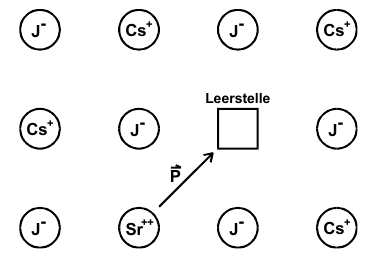
\includegraphics[height=6cm]{pics/Dipole.png}
  \caption{Mit \ce{Sr2+} dotiertes Cäsiumjodid \ce{CsJ} zur Darstellung von elektrischen Dipolen in Ionenkristallen. \cite{anleitung}}
  \label{fig:Dipol}
\end{figure}
\FloatBarrier

Die Richtung der Dipole hängt hierbei von der Verbindungsachse zwischen den Störstellen im Gitter ab, sie ist also quantisiert.
Solange die Temperatur des Kristalls unter \SI{500}{\celsius} ist, verändert sich die Dipolrichtung ausschließlich durch Leerstellendiffusion.
Dazu muss eine Potentialschwelle überwunden werden, die von dem räumlich periodischen Verlauf des Gitterpotentials abhängt.
Die nötige Energie ist die materialspezifische Aktivierungsenergie $W$.
Die Anzahl der Dipole, die durch thermische Fluktuationen genug Energie besitzen, um sich umzuorientieren, ist laut der Boltzmann-Statistik proportional zu $\exp(-W/\symup{k_b}T)$ pro Zeiteinheit.
Wird diese Fluktuation als Frequenz interpretiert, ergibt sich die mittlere Zeit zwischen zwei Orientierungen zu
\begin{equation}
    \label{eqn:Relaxzeit}
    \tau(T) = \tau_0 \exp\left(\frac{W}{\symup{k_B} T}\right)
\end{equation}
mit $\tau_0$ als charakteristische Relaxationszeit, $\symup{k_B}$ für die Boltzmann-Konstante und $T$ für die Temperatur.

Die zu untersuchende Probe dient als Dielektrikum eines Plattenkondensatoren, an dem vorerst eine Gleichspannung angelegt ist.
Durch das elektrische Feld werden einige Dipole in Feldrichtung ausgelenkt, die restlichen Dipole, wegen thermischer Gitterbausteinbewegung, zeigen
in andere Richtungen. Insgesamt zeigt also nur ein Bruchteil $y$ der Dipole in Feldrichtung.
Dieser Bruchteil lässt sich durch die Funktion
\begin{equation}
    \label{:eqn:dipolgesamtheit}
    y(T)=\frac{pE}{3\symup{k_B}T}
\end{equation}
ausdrücken.
Hierbei steht $p$ für die Dipolstärke und $E$ für die elektrische Feldstärke.

Während diese ausgerichteten Dipole wieder eine statistische Raumverteilung annehmen, was als Dipolrelaxation bezeichnet wird, ist ein Depolarisationsstrom messbar.
Der schematische Verlauf dieses Stromes ist in Abbildung \ref{fig:Strom} zu sehen.
Die Depolarisationsstromdichte $j(T)$ setzt sich als Produkt aus dem Anteil $y$ der bei der Polarisationstemperatur $T_\text{p}$ orientierten Dipole, dem Dipolmoment $p$ und der Zahl $\symup{d}N/\symup{d}t$
der pro Zeit und Volumeneinheit relaxierenden Dipole zusammen:
\begin{align*}
        j(T)=& y(T_{\symup{p}})\cdot p\cdot \frac{\symup{d}N}{\symup{d}t}\\
        =&\frac{p^2E}{3 \symup{k_B} T_\symup{p}}\frac{\symup{d}N}{\symup{d}t}.
\end{align*}
Weil die Dipolrelaxation ein thermisch aktivierter Prozess ist, ist $\symup{d}N/\symup{d}t$ proportional zur Anzahl $N$ der orientierten Dipole multipliziert mit der Relaxationsfrequenz $1/\tau$:
\begin{equation*}
    \frac{\symup{d}N}{\symup{d}t}=\frac{-N}{\tau(T)}.
\end{equation*}
Die Lösung für $N$ ist
\begin{equation*}
    N=N_{\symup{p}} \exp\left(-\frac{1}{h}\int_{T_{\symup{0}}}^{T}\frac{\symup{d}T'}{\tau(T')}\right),
\end{equation*}
wenn die Heizrate $h=\symup{d}T/\symup{d}t}=\text{const}$ ist.
$N_{\symup{p}}$ ist die Zahl der zu Beginn des Aufheizens (Zeitpunkt $t_{\symup{0}}$ und Temperatur $T_{\symup{0}}$) vorhandenden, orientierten Dipole pro Volumeneinheit.
Werden alle Ausdrücke zusammengefasst und umgeformt, wird die Stromdichte durch
\begin{equation}
\label{eqn:Stromdichte}
    j(T)=\frac{p^2 E N_{\symup{p}}}{3 \symup{k_B} T_{\symup{p}}\tau_0}\exp\left(-\frac{1}{h\tau_0}\int_{T_{\symup{0}}}^{T}\exp\left(\frac{-W}{\symup{k_B}T'}\right)\symup{d}T'\right)\exp\left(\frac{-W}{\symup{k_B}T}\right)
\end{equation}
beschrieben.
\begin{figure}[htb]
    \centering
    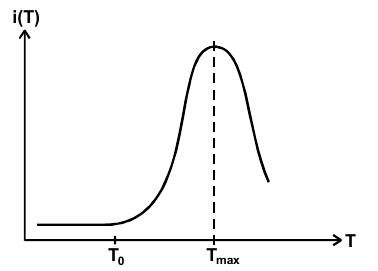
\includegraphics[height=6cm]{pics/Strom.png}
    \caption{Depolarisationsstrom in Abhängigkeit von der Temperatur. \cite{anleitung}}
    \label{fig:Strom}
\end{figure}
\FloatBarrier
Für den Anfangsteil der Depolarisationskurve genügt die Näherung
\begin{equation}
    j(T)=\frac{p^2 E N_{\symup{p}}}{3 \symup{k_B} T_{\symup{p}}\tau_0}\exp\left(\frac{-W}{\symup{k_B}T}\right).    
\end{equation}
Wird die Polarisation $P$ der Probe untersucht, ist es möglich $W$ genauer zu bestimmen, da der gesamte Kurvenverlauf analysiert wird.
$P$ ist gleich dem Gesamtdipolmoment pro Volumeneinheit und proportional zur Zahl der orientierten Dipole.
Wie vorher ist somit $\symup{d}P/\symup{d}t$ gleich der Anzahl der orientierten Dipole multipliziert mit der Relaxationsfrequenz als Proportionalitätsfaktor:
\begin{equation*}
    \frac{\symup{d}P}{\symup{d}t}=-\frac{P(t)}{\tau(T(t))}.
\end{equation*}
Der durch die Dipolrelaxation erzeugte Strom $i(t)$, ist gegeben durch
\begin{equation*}
    i(t)=F\frac{\symup{d}P}{\symup{d}t}
\end{equation*}
mit $F$ als Probendurchschnitt.
Nach einer Integration folgt
\begin{equation*}
    \int_{t(T)}^{\infty} i(t)\symup{d}t=-F P(t).
\end{equation*}
Weil $T$ eine lineare Funktion von $t$ ist, folgt die Beziehung
\begin{equation*}
\tau(T)=\frac{\int_{T}^{\infty }i(T')\symup{d}T'}{b i(T)}
\end{equation*}
aus den vorherigen Gleichungen.
Unter Berücksichtigung von \eqref{eqn:Relaxzeit} gilt
\begin{equation}
    \frac{W}{\symup{k_B}T}=\ln\frac{\int_T^\infty i(T')\symup{d}T'}{i(T)\tau_0 h}.
\end{equation}
Durch eine Regression wird $W$ schließlich ermittelt.
Aus dem Maximum von \eqref{eqn:Stromdichte} folgt die Relaxationszeit $\tau_0$ durch
\begin{equation}
    \label{eqn:tau0}
    \tau_0 = \frac{\symup{k_B}T_\text{max}^2}{W \cdot h} \exp\left(-\frac{W}{\symup{k_B}T_\text{max}} \right).
\end{equation}
$T_\text{max}$ ist die Temperatur bei der der größte Strom fließt (siehe Abb. \ref{fig:Strom}). 
% \begin{figure}[htb]
%   \centering
%   \includegraphics[height=5.5cm]{content/Bild.png}
%   \caption{Bilduterschrift}
%   \label{fig:Bild}
% \end{figure}

% \subsection{Unterkapitel}
% \label{sec:UnterKapitel}

% \begin{equation}
% Für Formeln
%   \label{eqn:Formel}
% \end{equation}
\FloatBarrier